\documentclass[11pt]{article}

\usepackage[letterpaper,bindingoffset=0.2in,
            left=1in,right=1in,top=1in,bottom=1in,
            footskip=.25in]{geometry}

\usepackage{hyperref}
	\hypersetup{
			colorlinks=true,
			linkcolor=black,
			filecolor=magenta,      
			urlcolor=blue,
	}
	
\usepackage{graphicx}
	\graphicspath{ {images/} }
	
\usepackage{subcaption}
	
\begin{document}


\title{COMP SCI 5401 FS2017 Assignment 1c}
\author{Stuart Miller\\\href{mailto:sm67c@mst.edu}{sm67c@mst.edu}}
\maketitle


\section{Overview}\label{sect:overview}

Assignment 1c presented a great many parameters to test. As more techniques are introduced, it becomes more and more difficult to distinguish a genuinely "`good"' parameter value as one can never be entirely sure if it was solely one value that resulted in a change in fitness landscape, a combination of multiple values, or perhaps the order of calls to the random number generator came out more favorably. Therefore, in this assignment, it has been attempted to isolate parameters being tested and pick favorable and reasonably values to the parameters not immediately relevant.

As a precursor, the entirety of this assignment will make use of n-point crossovers and random reset mutations. Although other operators are implemented in the codebase, these two have been set to be self-adaptive in Bonus 2. For consistency with the runs in the Bonus section, even when self-adaptability is turned off, the analysis will still use only these two operators. For initial values and non adaptive states, the operators will be fixed at three crossover points and a 12\% mutation chance. These are values that were determined to be beneficial in Assignment 1b. Furthermore, survival strategy will always be set to comma \((\mu,\lambda)\) and selection will be k-tournaments with moderate selective pressure.

Furthermore, box plots were generated for each test run graphed below. As this totals to a rather large number of boxplots, they have not been pictured in this report. Instead, they can be viewed in ./doc/images/assn1c\_boxplot\_*.png.


\section{Penalty Coefficient}\label{sect:penalty}

To test the penalty coefficient, two control sets were run where invalid placements were solved by random replacements and then a repair. The penalty function was then implemented, with static weights of 1.0, 2.0, and 5.0, respectively.

\begin{figure}[h]
\begin{minipage}{.5\textwidth}
  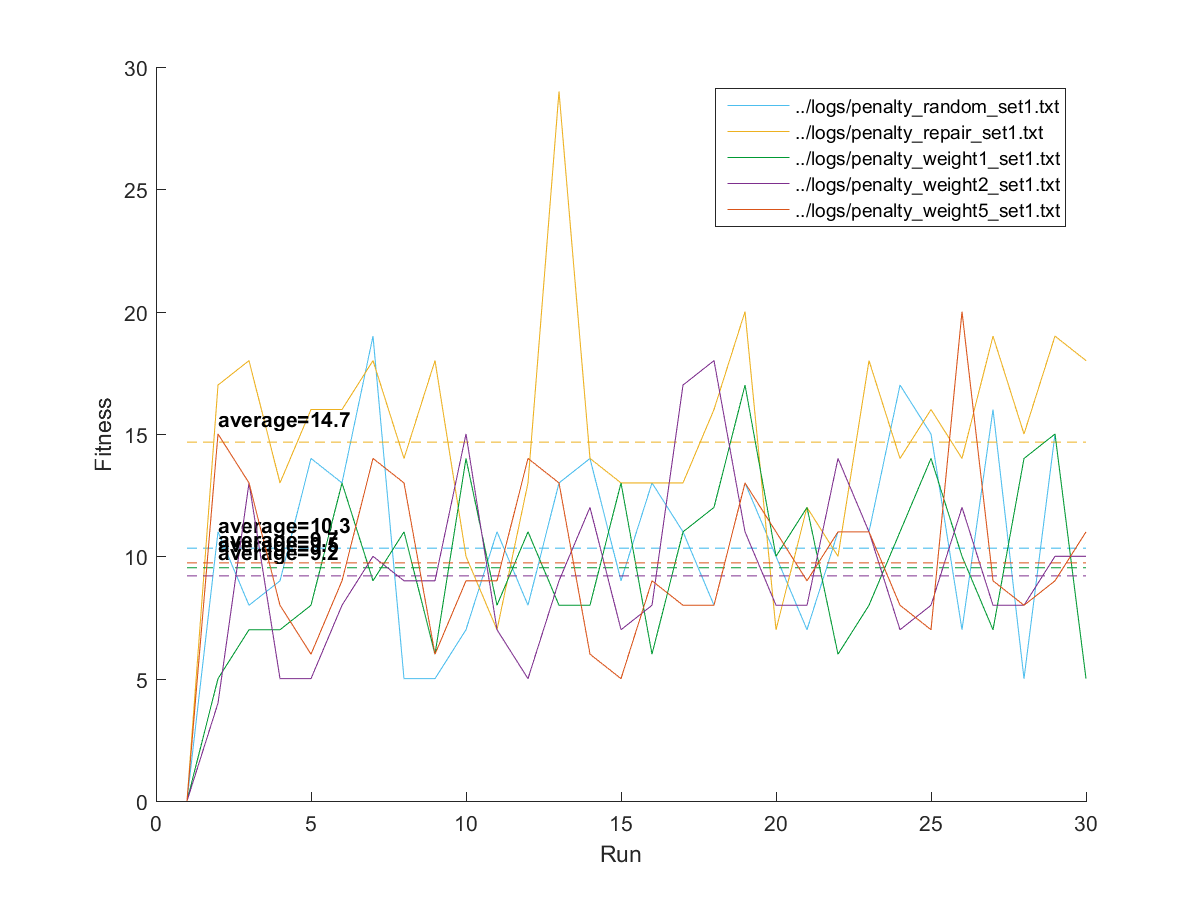
\includegraphics[width=3.25in]{assn1c_graph_penalty_set1.png}
  \captionof{figure}{Penalty Weights, 50Shapes.txt}
  \label{fig:penaltyset1}
\end{minipage}%
\begin{minipage}{.5\textwidth}
  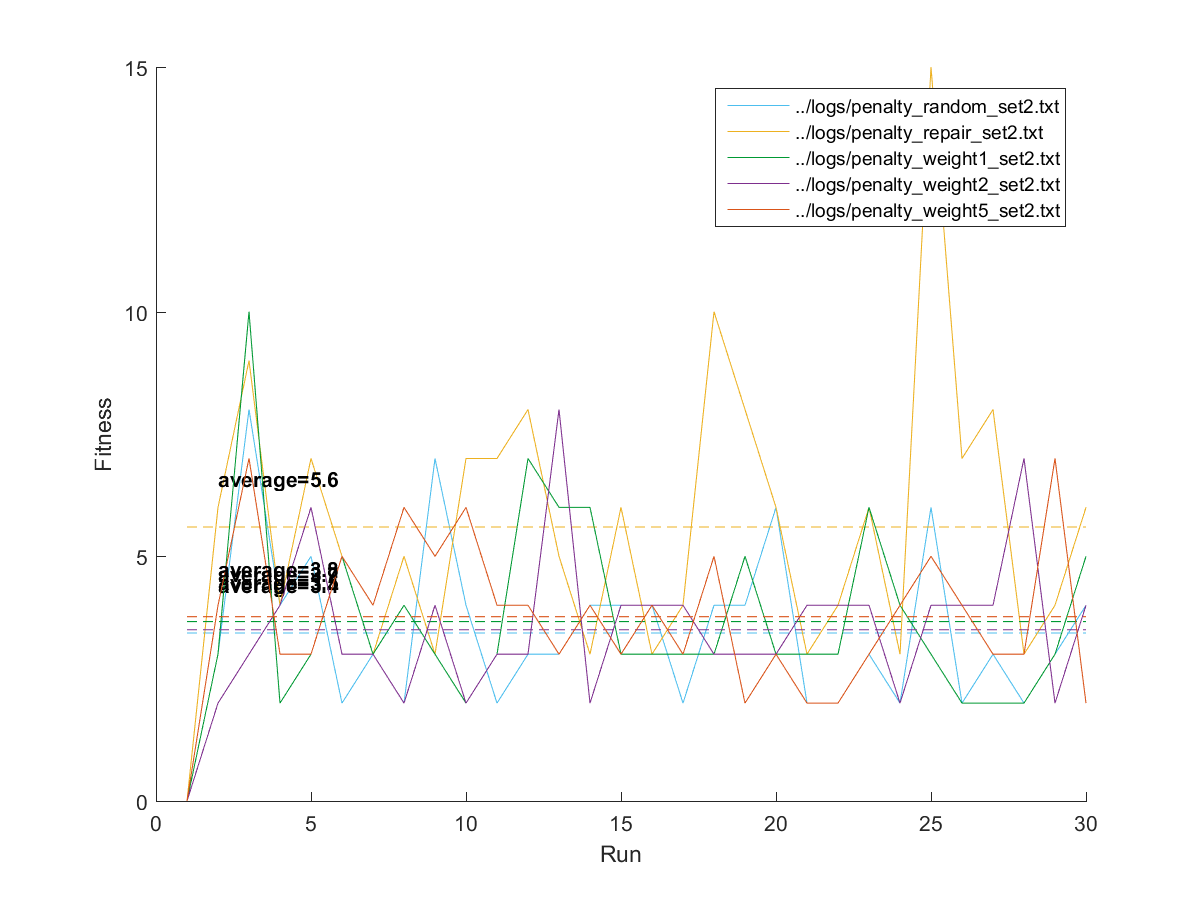
\includegraphics[width=3.25in]{assn1c_graph_penalty_set2.png}
  \captionof{figure}{Penalty Weights, 100Shapes.txt}
  \label{fig:penaltyset2}
\end{minipage}
\end{figure}
\begin{figure}[h]
	\centering
  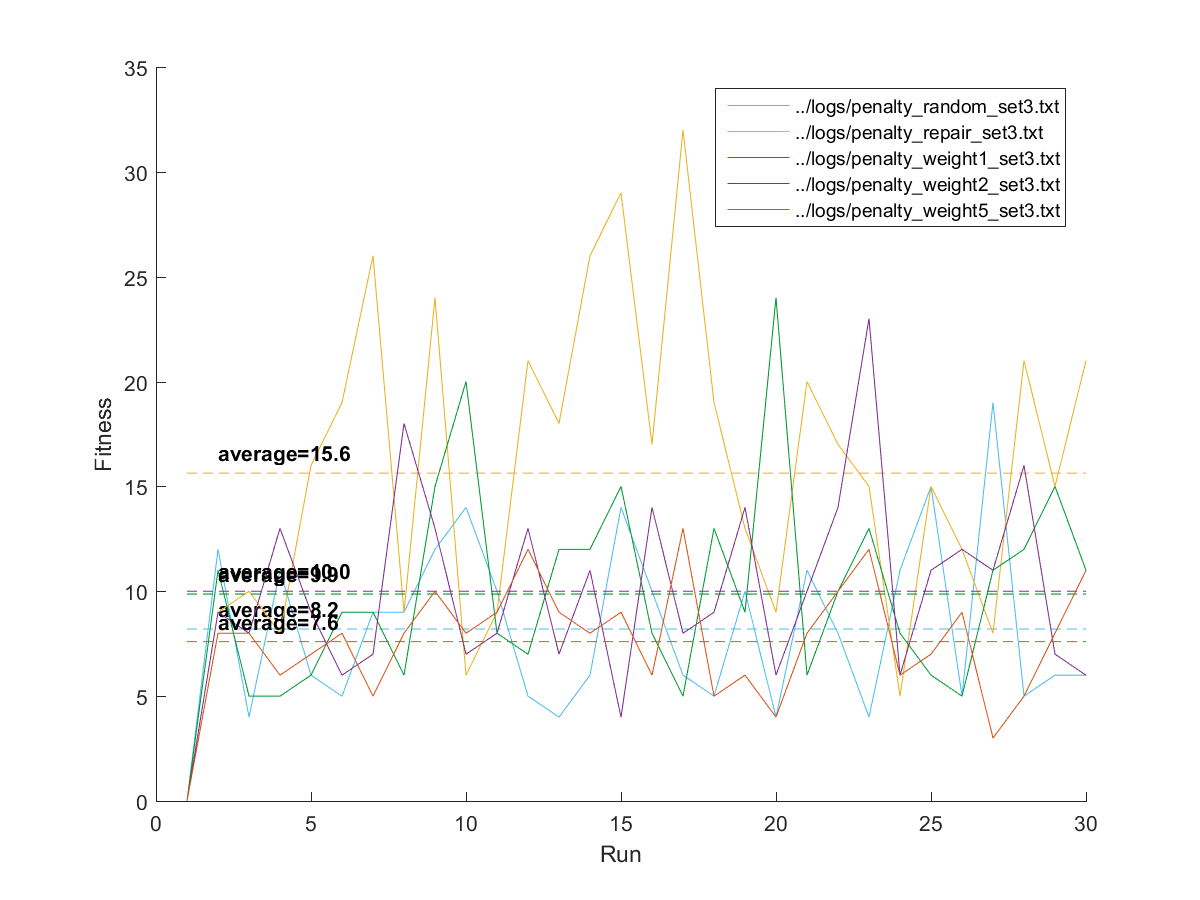
\includegraphics[width=3.25in]{assn1c_graph_penalty_set3.png}
  \captionof{figure}{Penalty Weights, 100ShapesComplex.txt}
  \label{fig:penaltyset3}
\end{figure}

As the graph in Figures \ref{fig:penaltyset1}, \ref{fig:penaltyset2}, and \ref{fig:penaltyset3} all show, the penalty weight functions shows significantly lower fitness values than other methods. This is to be expected for intermediate solutions, but the best solution shouldn't have any penalty. Additionally, the fact the the different weights returned the same max fitness shows that this may not be an optimal strategy for this problem. It is worth noting that numerous evolutionary strategy were tried and this combination yielded the best and most consistent results.


\newpage
\section{Self-Adaptive Parameter}\label{sect:selfadaptive}

To test self-adaptability, the number of crossover points \textit{n} was set to be adaptable. For offspring created, there was an equivalent random chance of inheriting each parent's \textit{n}. Additionally, \textit{n} had a small chance to mutate (equivalent to the genetic mutation rate) by $\pm$1. For analysis, the mutation rate was averaged across all member of the population for each generation.

As it was determined in Section \ref{sect:penalty}, the penalty function yields no great benefit for this problem, so the repair function method was used here instead. The other parameters were kept the same as in section \ref{sect:penalty}.

\begin{figure}[h]
\begin{minipage}{.5\textwidth}
	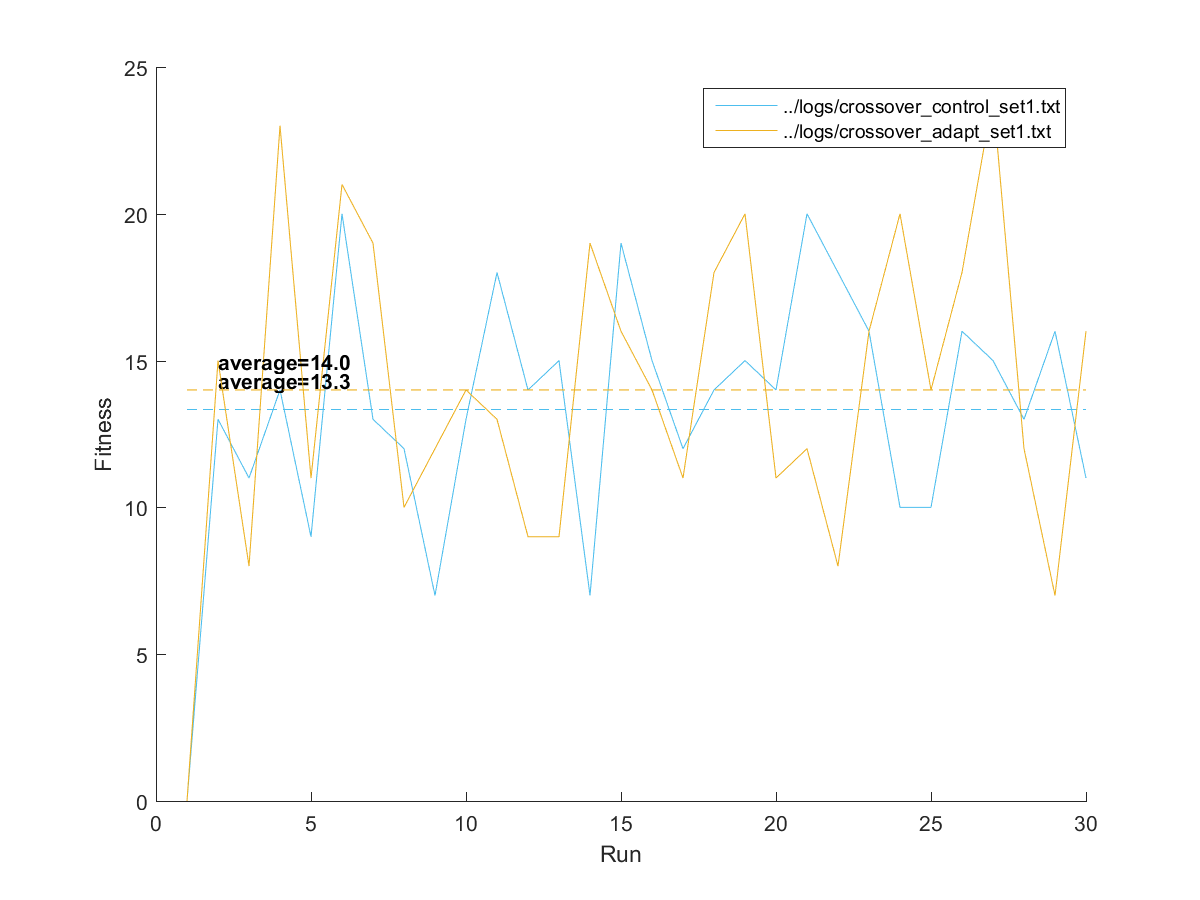
\includegraphics[width=3.25in]{assn1c_graph_crossover_adapt_set1.png}
  \captionof{figure}{Adaptive Crossovers, 50Shapes.txt}
  \label{fig:crossoverset1}
\end{minipage}%
\begin{minipage}{.5\textwidth}
  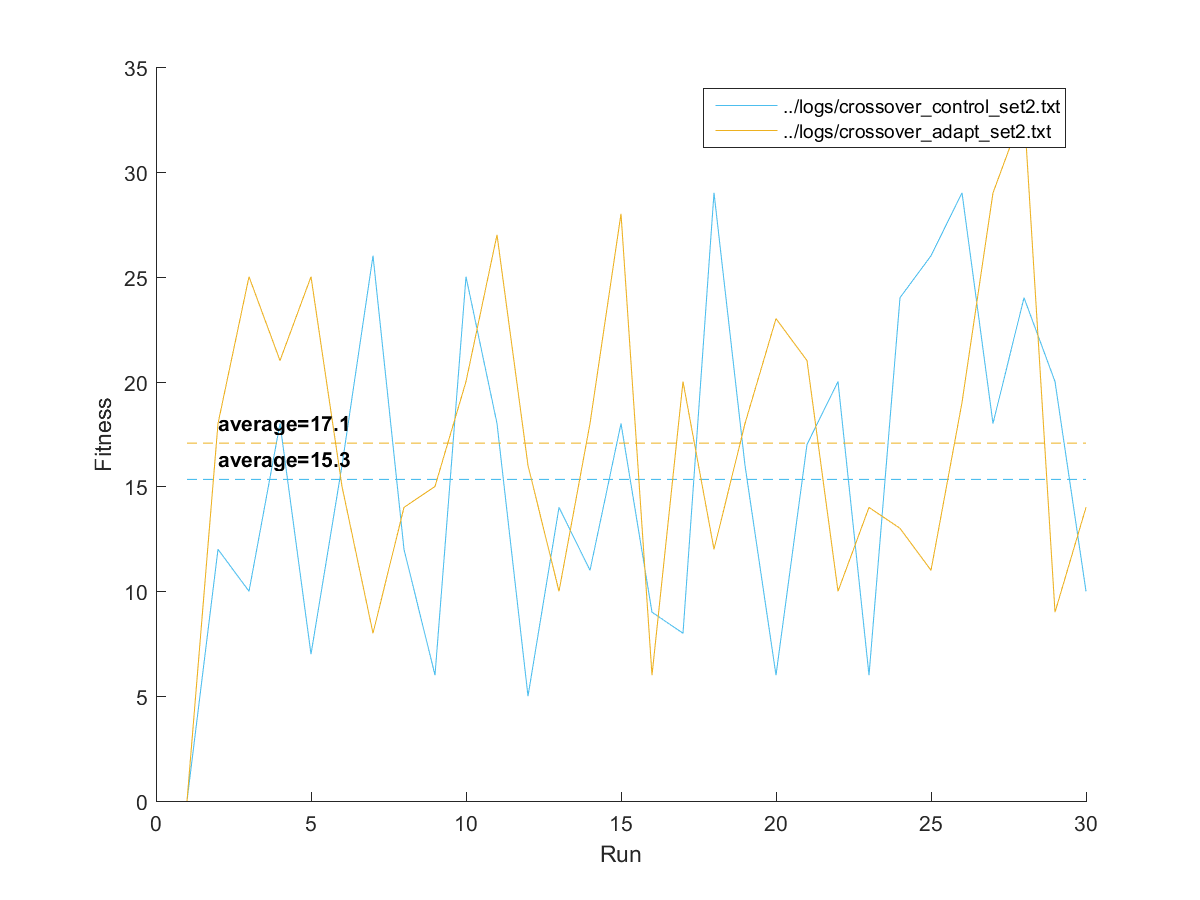
\includegraphics[width=3.25in]{assn1c_graph_crossover_adapt_set2.png}
  \captionof{figure}{Adaptive Crossovers, 100Shapes.txt}
  \label{fig:crossoverset2}
\end{minipage}
\end{figure}
\begin{figure}[h]
	\centering
  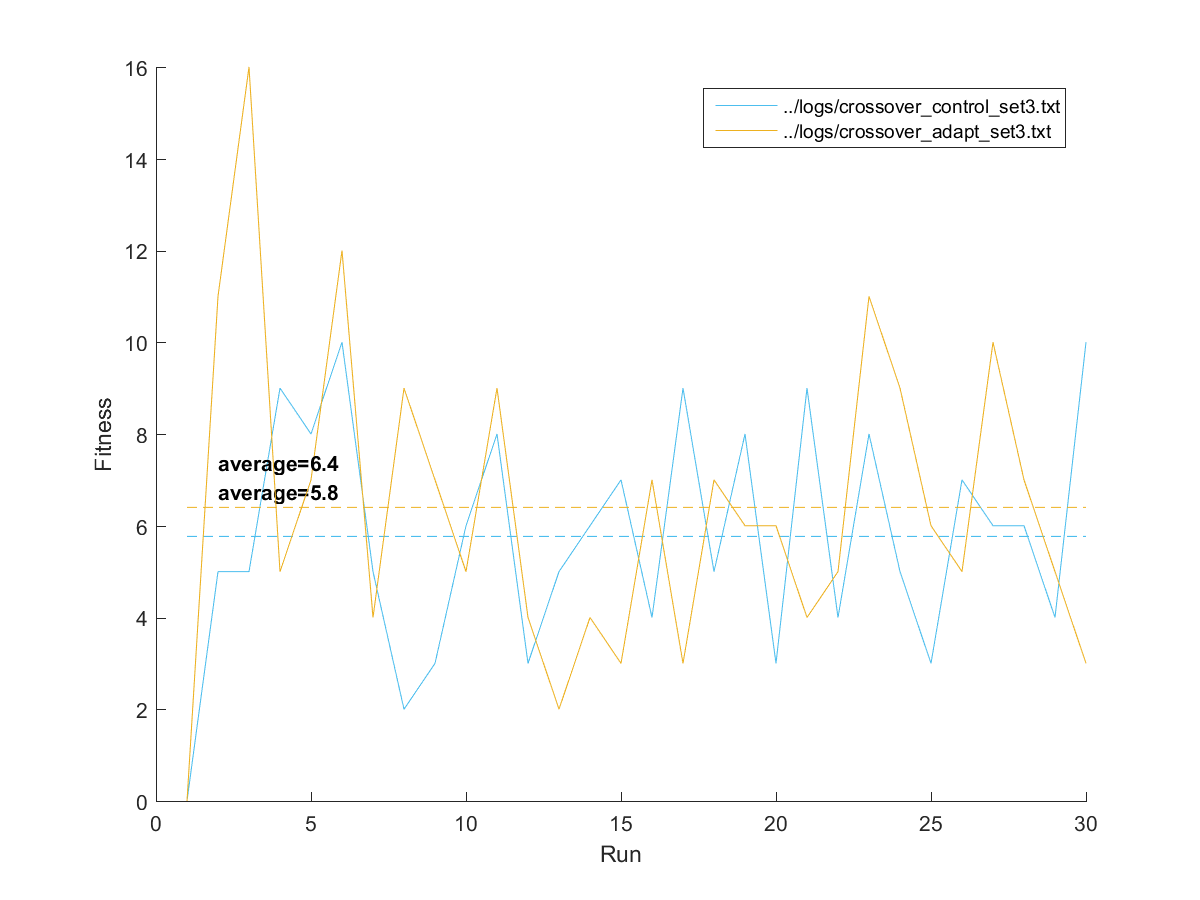
\includegraphics[width=3.25in]{assn1c_graph_crossover_adapt_set3.png}
  \captionof{figure}{Adaptive Crossovers, 100ShapesComplex.txt}
  \label{fig:crossoverset3}
\end{figure}

As figures \ref{fig:crossoverset1}, \ref{fig:crossoverset2}, and \ref{fig:crossoverset3} all show, allowing crossovers to self-adapt has a significant improvement on the average best fitness. It is also interesting to worth noting that while each instance started at three crossover points, some runs took this number higher, and some drove it lower. Examining the log (located in the ./logs/ directory) shows no consistent trend. It can only be assumed that each run's random initialization took it to a different area of the fitness landscape where more or less crossovers were desirable.


\section{Bonus 1}


\section{Bonus 2}


\end{document}